\let\negmedspace\undefined
\let\negthickspace\undefined
\documentclass[journal]{IEEEtran}
\usepackage[a5paper, margin=10mm, onecolumn]{geometry}
%\usepackage{lmodern} % Ensure lmodern is loaded for pdflatex
\usepackage{tfrupee} % Include tfrupee package

\setlength{\headheight}{1cm} % Set the height of the header box
\setlength{\headsep}{0mm}     % Set the distance between the header box and the top of the text

\usepackage{gvv-book}
\usepackage{gvv}
\usepackage{cite}
\usepackage{amsmath,amssymb,amsfonts,amsthm}
\usepackage{algorithmic}
\usepackage{graphicx}
\usepackage{textcomp}
\usepackage{xcolor}
\usepackage{txfonts}
\usepackage{listings}
\usepackage{enumitem}
\usepackage{mathtools}
\usepackage{gensymb}
\usepackage{comment}
\usepackage[breaklinks=true]{hyperref}
\usepackage{tkz-euclide} 
\usepackage{listings}
% \usepackage{gvv}                                        
\def\inputGnumericTable{}                                 
\usepackage[latin1]{inputenc}                                
\usepackage{color}                                            
\usepackage{array}                                            
\usepackage{longtable}                                       
\usepackage{calc}                                             
\usepackage{multirow}                                         
\usepackage{hhline}                                           
\usepackage{ifthen}                                           
\usepackage{lscape}
\begin{document}

\bibliographystyle{IEEEtran}
\vspace{3cm}

\title{1.1.2.16}
\author{AI24BTECH11027 - R Sumanth}
% \maketitle
% \newpage
% \bigskip
{\let\newpage\relax\maketitle}

\renewcommand{\thefigure}{\theenumi}
\renewcommand{\thetable}{\theenumi}
\setlength{\intextsep}{10pt} % Space between text and floats



\textbf{Questions:} $\vec{(-1,2,1)}$, $\vec{(1,-2,5)}$, $\vec{(4,-7,8)}$ and $\vec{(2,-3,4)}$ are the vertices of a parallelogram.

\solution

properties : opposite sides of parallelogram are equal.\\

$\Vec{A}(-1, 2, 1), \quad \vec{B}(1, -2, 5), \quad \vec{C}(4, -7, 8), \quad \vec{D}(2, -3, 4)$ \\


$\overrightarrow{AB}= B - A =\vec{(1 - (-1), -2 - 2, 5 - 1)} =\vec{(2, -4, 4)}$ \\

$\overrightarrow{BC} = C - B = \vec{(4 - 1, -7 - (-2), 8 - 5)} =\vec{(3, -5, 3)}$ \\

$\overrightarrow{CD} = D - C =\vec{(2 - 4, -3 - (-7), 4 - 8)} = \vec{(-2, 4, -4)}$ \\

$\overrightarrow{DA} = A - D = \vec{(-1 - 2, 2 - (-3), 1 - 4)} = \vec{(-3, 5, -3)}$ \\

Verify if $\overrightarrow{AB}$ is equal to $ \overrightarrow{CD} $ and $ \overrightarrow{BC} $ is equal to $ \overrightarrow{DA} $:

$\overrightarrow{AB} + \overrightarrow{CD} = \vec{(2, -4, 4)} + \vec{(-2, 4, -4)} = \vec{(0, 0, 0)}$ \\

$\overrightarrow{BC} + \overrightarrow{DA} = \vec{(3, -5, 3)} + \vec{(-3, 5, -3)} = \vec{(0, 0, 0)}$ \\

Since $\overrightarrow{AB} + \overrightarrow{CD} = 0 $ and $ \overrightarrow{BC} + \overrightarrow{DA} = 0 $, the quadrilateral formed by the points is a parallelogram.

\begin{figure}[h!]
   \centering
   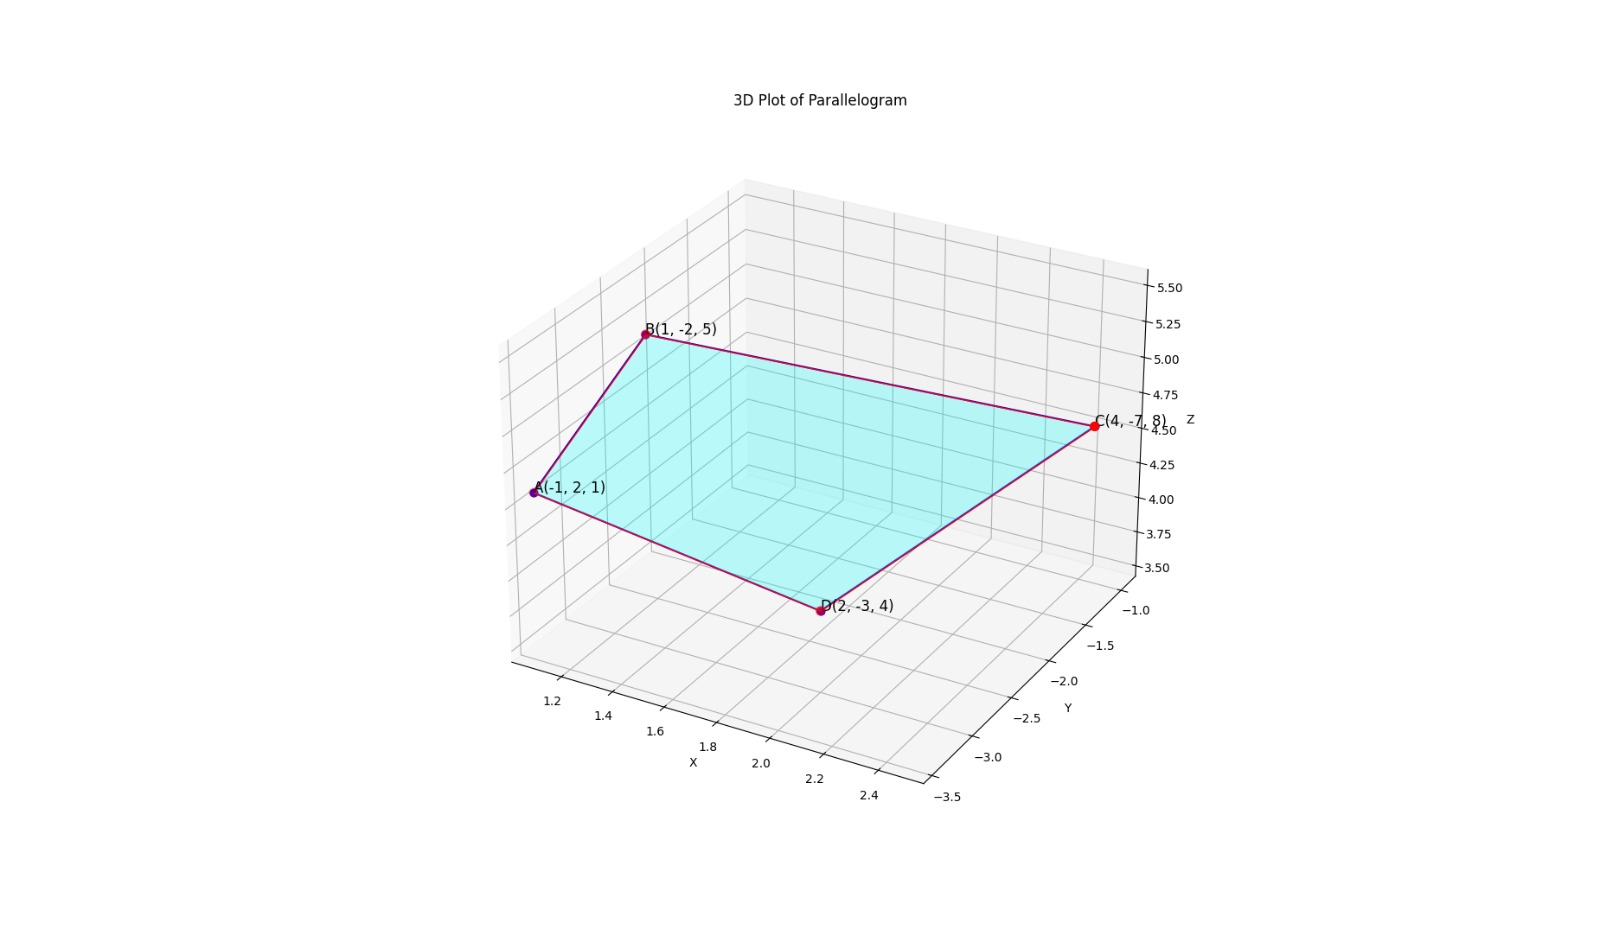
\includegraphics[width=0.7\linewidth]{IMG.jpg}
   \caption{Stem Plot of y\brak{n}}
     \label{stemplot}
\end{figure}

\numberwithin{equation}{enumi}
\numberwithin{figure}{enumi}
\renewcommand{\thetable}{\theenumi}



\end{document}  
